% CollecTF chapter

\chapter{CollecTF: a database of experimentally validated transcription
  factor-binding sites in Bacteria}

The binding of transcription factors (TF) to target sites in genomic DNA is a
defining element of transcriptional regulatory networks (TRN). Bacterial
transcription networks rely extensively on direct TF–DNA interactions and
display relatively lower complexity than their eukaryotic counterparts
\citep{wunderlich2009different, remenyi2004combinatorial}. This has generated
substantial interest in modeling and cataloging bacterial TF-binding site
interactions, leading to the emergence of several model organism-based
databases aimed at compiling TF-binding sites to define TRN and explore their
interplay with other cellular systems~\citep{salgado2013regulondb,
  jacques2005mtbreglist, pauling2012coryneregnet, sierro2008dbtbs}, as well as
two databases dedicated to compiling gene-regulation information across
multiple prokaryotic species~\citep{munch2005virtual,
  kazakov2007regtransbase}. In recent years, the development of high-throughput
techniques for the identification of TF-binding sites, like ChIP-Seq
\citep{mardis2007chip}, has led to a rising influx of data that challenges the
traditional manual curation process and the underlying definition of TF-binding
sites in current databases~\citep{salgado2013regulondb}. In turn, the increasing
availability of such data and the mounting evidence on the complexity of
TF-binding site recognition and regulatory logic in
Bacteria~\citep{hijum2009mechanisms, paul2007integration, barnard2004regulation}
have led to the proliferation of machine learning and comparative genomics
techniques to model TF-binding site interactions~\citep{narlikar2013mumod,
  maienschein2012improved, zwir2005dissecting}. These approaches require the
integration of genome-wide, multi-species knowledge on TF binding, using a
broader definition of TF-binding site and having direct access to the
experimental sources of evidence for each site. At present, cross-species
information is hard to compile and standardize across prokaryotic TF-binding
site databases. Different databases use different ranking systems for
experimental evidence, which is not always made directly accessible, and will
often combine experimentally supported sites with computational predictions, as
well as naturally occurring sites with artificially generated
ones. CollecTF~\citep{kilic2013collectf} seeks to address these issues and
complement existing databases by providing high-quality, transparent annotation
on naturally occurring TF-binding sites across the Bacteria domain, explicitly
integrating multiple sources of evidence and binding site definitions into a
highly accessible, machine readable and fully customizable database. In line
with previous initiatives~\citep{griffith2008oreganno}, CollecTF combines
in-house curation with direct submission from authors, and seeks to foster a
sustainable external submission model through its integration with NCBI RefSeq
\citep{pruitt2007ncbi}, UniProt KnowledgeBase~\citep{uniprot2014uniprot},
Evidence Ontology~\citep{chibucos2014standardized} and Gene
Ontology~\citep{gene2004gene}.

\section{Database Content}

CollecTF contains exclusively experimentally verified TF-binding sites
identified in natural DNA sequences. Historically, the definition for
TF-binding site has been associated to the presence of a well-defined
TF-binding motif, but in the last decade it has become increasingly apparent
that many TFs bind DNA without clear-cut sequence
determinants~\citep{hijum2009mechanisms, paul2007integration,
  barnard2004regulation}. To accommodate this diversity without losing the
high-quality annotation of motif determinants, CollecTF curators classify sites
as motif associated or non-motif associated. Motif associated sites are either
explicitly identified by authors as following a pre-established motif or shown
by means of detailed experimental work (e.g.\ site-directed mutagenesis) to
conform to a new motif. Non-motif associated sites are any DNA fragments
conclusively identified by the authors as bound to the TF;\ this includes ChIP
sites as reported by authors using a given peak-calling method and confidence
interval. Any quantitative information associated with sites (e.g.\ estimated
$K_d$) is also stored during curation, together with its range and a short
description of the quantitative technique. For ChIP data, additional
information on the experimental conditions and the ChIP protocol is also
compiled.

Experimental evidence of binding for a given genomic position may be
distributed across multiple reported sites of either type. Wherever a motif
associated site has been defined, CollecTF dynamically combines multiple
sources of evidence by arbitrarily defining a leader site and using two simple
pair-wise propagation rules. Evidence from two motif associated sites is
combined if the overlap between sites is more than 75\% of the combined site
length. Evidence from non-motif associated sites is integrated into a leader
site if they fully overlap any of the combined motif associated sites.

CollecTF was born with the goal of unifying and simplifying data collection on
TF-binding sites for comparative genomics and machine learning approaches. In
its initial release, CollecTF curators have focused on providing comprehensive,
domain-wide coverage for two TF families (LexA and Fur), as well as extensive
TF representation for bacterial clades, such as the \textit{Vibrio} and
\textit{Yersinia} genera and the \textit{Xanthomonadaceae} and
\textit{Pseudomonadaceae} families for which
abundant knowledge on the intertwined transcriptional regulation of virulence
is available in the literature but poorly represented in available
databases~\citep{matson2007regulatory}. Since its inception in 2013, CollecTF
has compiled over 9,750 experimentally-validated TF-binding sites, mapping to
more than 390 unique TF instances from over 240 transcription factors in over
100 bacterial species (Table~\ref{tab:collectf-stats}). This has situated
CollecTF at the forefront of transcription regulation databases in Bacteria,
rivaling the content and breadth of comparable initiatives, such as the
\textit{Escherichia coli}-centered RegulonDB~\citep{salgado2013regulondb} or the
prokaryotic-wide RegTransBase databases~\citep{kazakov2007regtransbase}.

\begin{table}
  \centering
  \caption{CollecTF statistics}
  \begin{tabular}{l r}
    \toprule
    Number of TFs & 244\\
    Number of TF instances (species-specific TFs) & 397\\
    Number of species & 318\\
    Number of curations & 865\\
    Number of binding sites & 9,795\\
    Number of publications & 2123 (45\% curated)\\
    \bottomrule
  \end{tabular}
  \label{tab:collectf-stats}
\end{table}

CollecTF plans to steadily increase its coverage by targeting other bacterial
groups of clinical and agricultural relevance not covered by organism-based
databases, such as the \textit{Xanthomonadaceae} or the
\textit{Pseudomonadaceae}, focusing on TF families with substantial
experimental support across multiple species, such as OmpR and LuxR, and
promoting direct author submissions on any transcriptional system/species.

\section{Curation Process}

%TODO: add database schema as appendix

The main goal of CollecTF is to provide high-quality annotation on
experimentally validated TF-binding sites in their genomic context. This is
accomplished through the manual curation of peer-reviewed literature with a
special focus on the experimental process used to identify TF-binding
sites. Curations may be initiated in-house by a team of curators specifically
trained on the experimental techniques used to determine TF-binding sites, or
by direct submission from authors. In all cases, curations are double-checked
by at least two curators following a well-defined set of guidelines before
inclusion in the database. Given its fundamental importance, the curation
process is the central element of the relational database structure of CollecTF
(Figure~\ref{fig:data-structure}). A curation essentially establishes a link
from a TF and a number of sites as reported in a scientific publication to a
set of genome positions and a protein accession in the UniProtKB
database~\citep{uniprot2014uniprot}. The mapping process involves an automated
search of reported sites in the target reference sequence and manual
verification of their genomic location by the curator. Exact matching sequences
for each binding site are first identified in the reference genome and their
genomic location is reported to the curator together with information on the
functional annotation of nearby genes. The curator uses this contextual
information to validate the correspondence between identified genome positions
and reported sites. For reported sites without exact matches in the genome, a
search allowing up to two mismatches is performed. Identified sequences are
again annotated with contextual information, ranked using a position-specific
weight matrix derived from the list of reported sites and presented to the
curator for manual verification. For any given curation, at least 90\% of the
reported sites must have exact matches in the reference genome in order for the
mapping to be accepted. Otherwise, the submitted data is stored but not
submitted to other major biological sequence databases. Most importantly, for
each TF-site pair the curation process also determines all the techniques used
to identify the site and its regulatory role on nearby genes, and generates a
summary description of the experimental process. CollecTF distinguishes between
two primary experimental sources: direct evidence of binding and evidence of
TF-mediated regulation. In silico techniques are annotated as complementary
sources in the experimental process, but are not admitted as the single source
of evidence for a record. CollecTF does not rank experimental
techniques. Instead, it provides direct queryable access to the experimental
support, providing users with full control over quality standards of retrieved
data.

\begin{figure}
  \centering
  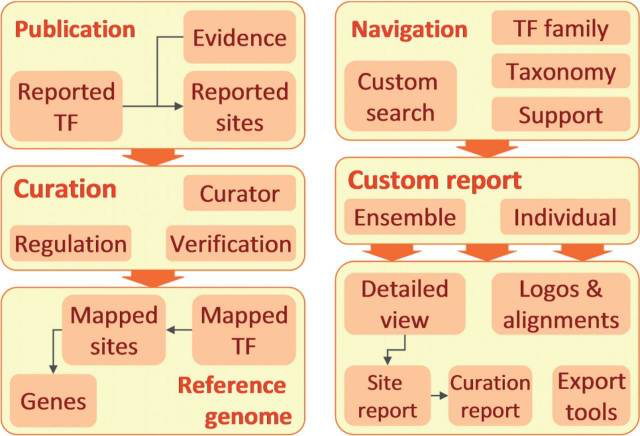
\includegraphics[width=0.8\textwidth]{figures/chapter2/data-structure}
  \caption{Schematic representation illustrating the CollecTF data structure,
    curation and navigation processes. (Left panel) The curation table is the
    pivotal element of the relational design in CollecTF, providing a central
    link to all the other tables in the database and establishing a link
    between reported TF-binding sites, the evidence supporting them, their
    regulatory effects on genes and their mapped instances in a reference
    genome. (Right panel) Navigation is initiated by browsing or customized
    search, leading to a dynamically generated report that can be cumulative or
    individualized for each TF/species pair. Motif alignments and logos are
    provided for visualization, together with export functions to FASTA and
    flat-file formats. Users can link out to specific site reports and link-out
    to curation reports to evaluate all the supporting evidence for reported
    sites and the genome mapping process.}
\label{fig:data-structure}
\end{figure}

\section{Navigation and Availability}

\subsection{Customizable access}

CollecTF (\url{http://collectf.org}) is designed to maximize ease of access to
TF-binding site data in both human- and machine-readable formats. Users can
browse the database taxonomically, by TF family or by experimental techniques,
or search clades and TF families for sites with specific types of experimental
support (e.g.\ all Fur sites in \textit{Pseudomonas} identified through
mobility shift assays). Users can elicit reports at any time during browsing or
searching, and have the option of condensing the report or reporting by
individual species/TFs. Instead of relying on pre-computed motif
representations, motif associated sites are realigned dynamically with LASAGNA
and displayed with WebLogo~\citep{crooks2004weblogo, lee2013lasagna}, providing
a fluid representation of TF-binding motifs that incorporates all the available
sources of evidence selected by the user (Figure~\ref{fig:weblogo}). All report
pages offer a detailed view of TF-binding sites in their genomic context with
out-links to site description and gene NCBI accessions, as well as export
options to FASTA, flat-file CSV and ARFF sequence formats and multiple
position-specific matrix formats (Figure~\ref{fig:motif-reports}).

All data stored in CollecTF is directly accessible through
navigation. Navigating from main report pages, users may inspect the individual
site instances contributing support for a specific leader site in a motif
alignment or access the curation record including curation notes, out-links to
external databases for supporting evidence and both the originally reported and
the genome-mapped data (Figure~\ref{fig:individual-site}). Flat-file versions
of CollecTF primary tables are generated periodically and made freely available
for download.

\begin{figure}
  \centering
  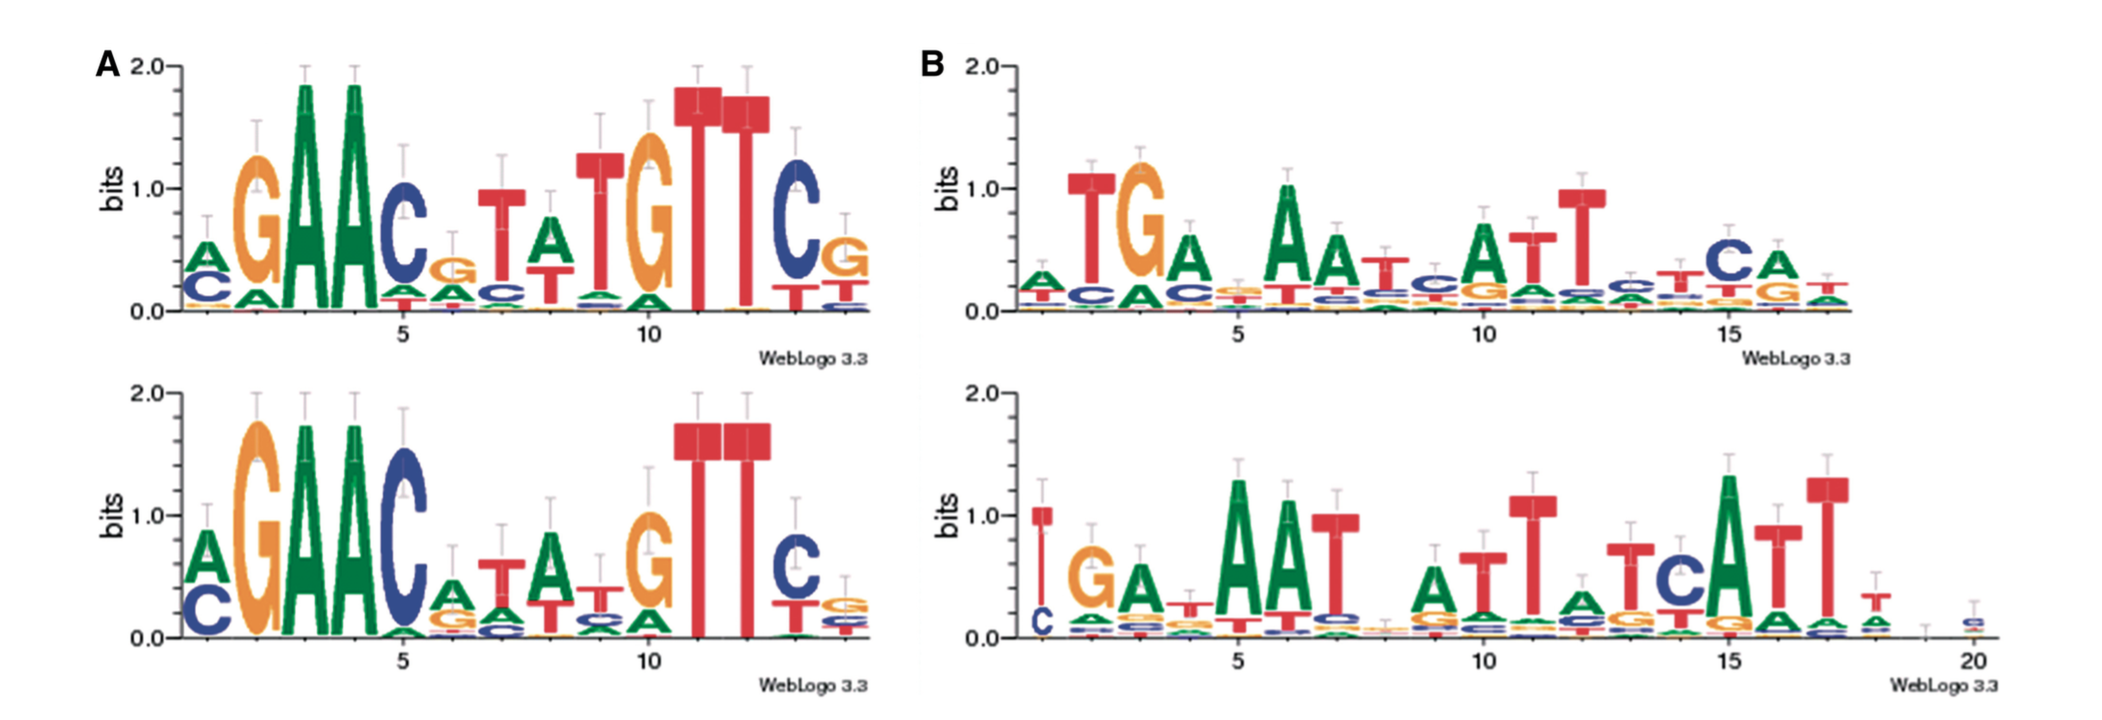
\includegraphics[width=\textwidth]{figures/chapter2/weblogo}
  \caption{(A) Sequence logo for LexA-binding sites in the Firmicutes (top) and
    in \textit{Bacillus subtilis} (bottom). (B) Sequence logo for Fur-binding
    sites with experimental evidence of binding (top) or experimental evidence
    of regulation (bottom). Both examples are extracted from dynamically
    generated CollecTF reports and illustrate the ability to customize queries
    and the fluidity inherent to the concept of TF-binding motif in CollecTF.}
\label{fig:weblogo}
\end{figure}

\begin{figure}
  \centering
  \begin{subfigure}{0.9\textwidth}
  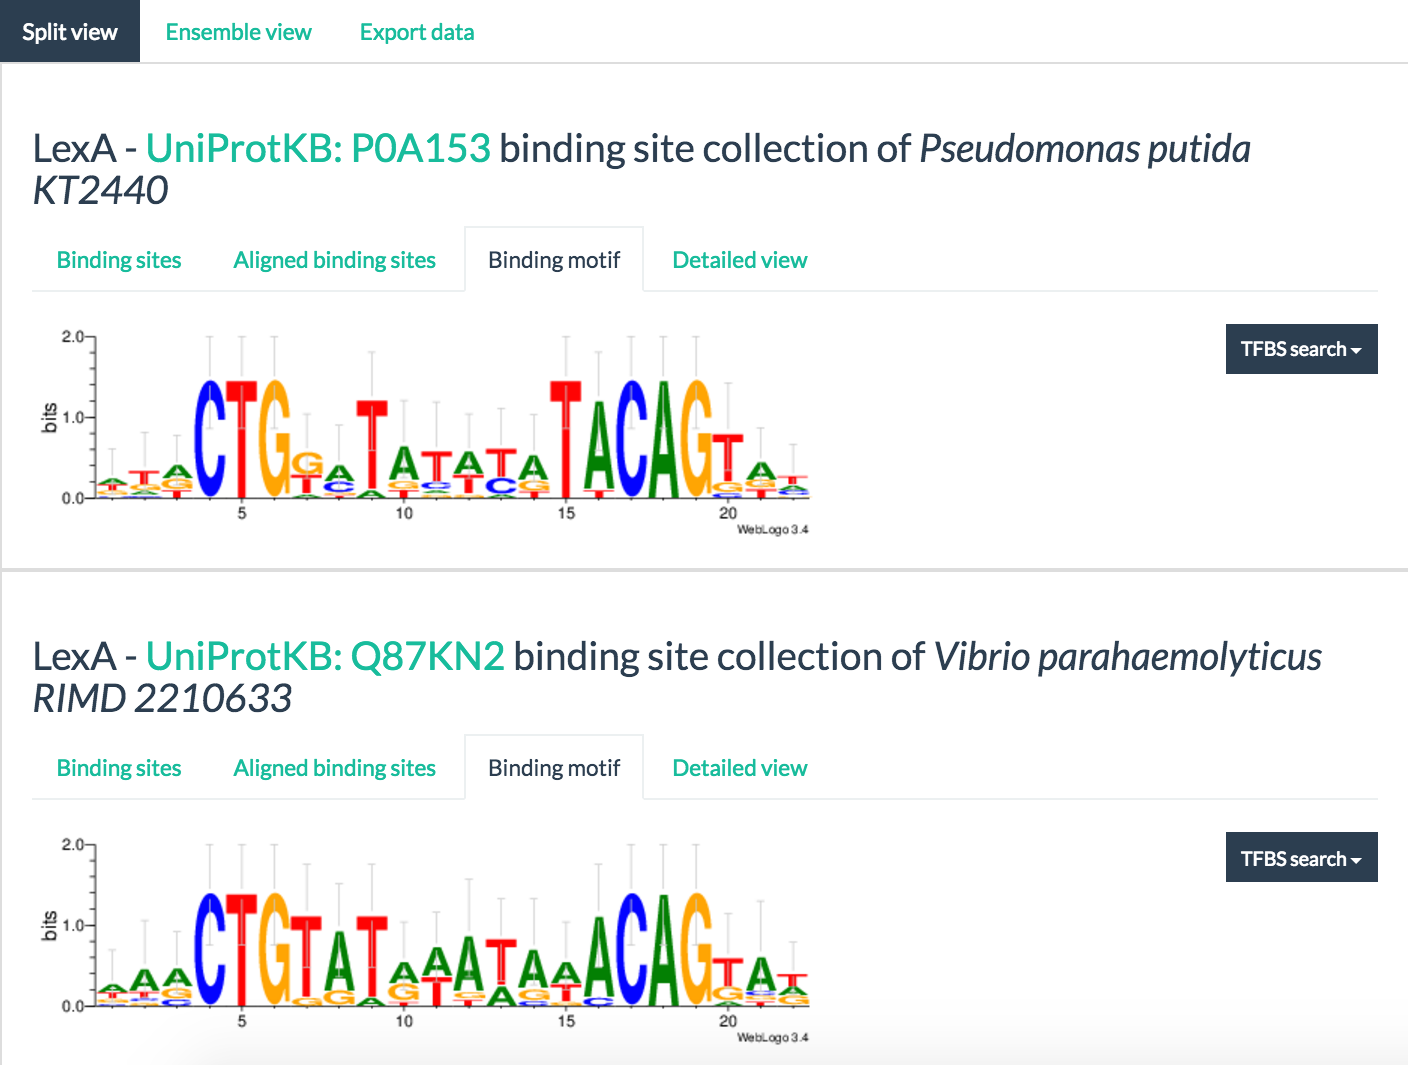
\includegraphics[width=1\textwidth]{figures/chapter2/report-split-view}
  \caption{}
  \end{subfigure}

  \begin{subfigure}{0.9\textwidth}
  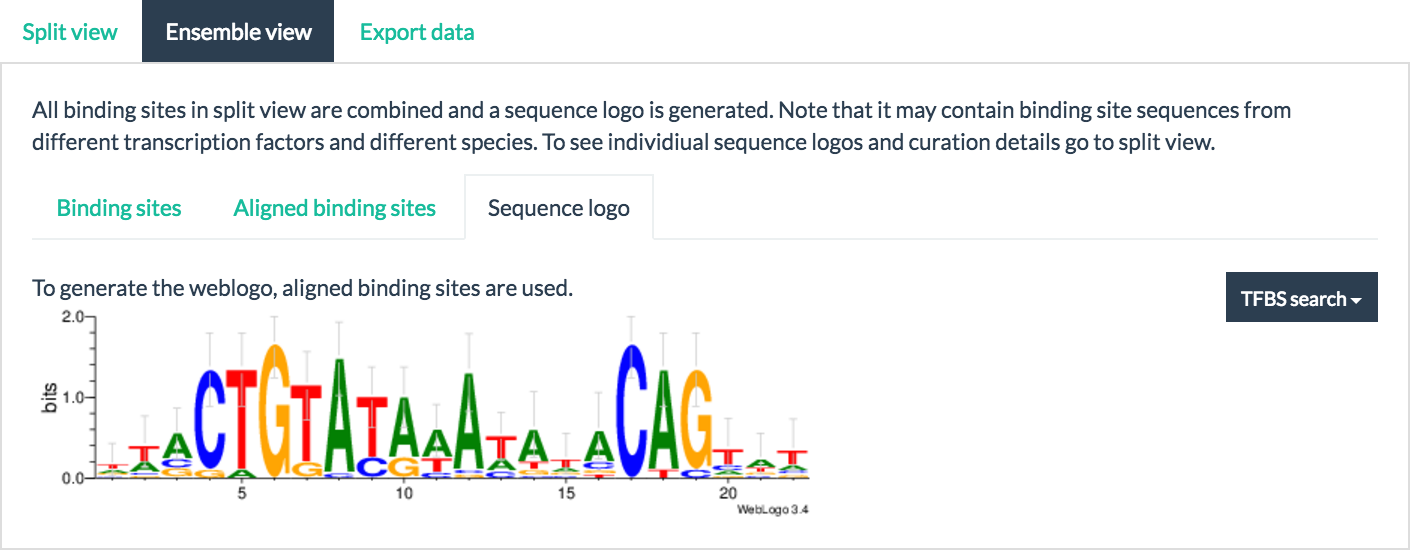
\includegraphics[width=1\textwidth]{figures/chapter2/report-ensemble-view}
  \caption{}
  \end{subfigure}

  \caption{Screenshot of a dynamically generated report of LexA-binding sites
    in the Gammaproteobacteria as (a) individual TF/species pair (split)
    reports and (b) an ensemble report integrating all Gammaproteobacteria
    sites of LexA.}
\label{fig:motif-reports}
\end{figure}

\begin{figure}
  \centering
  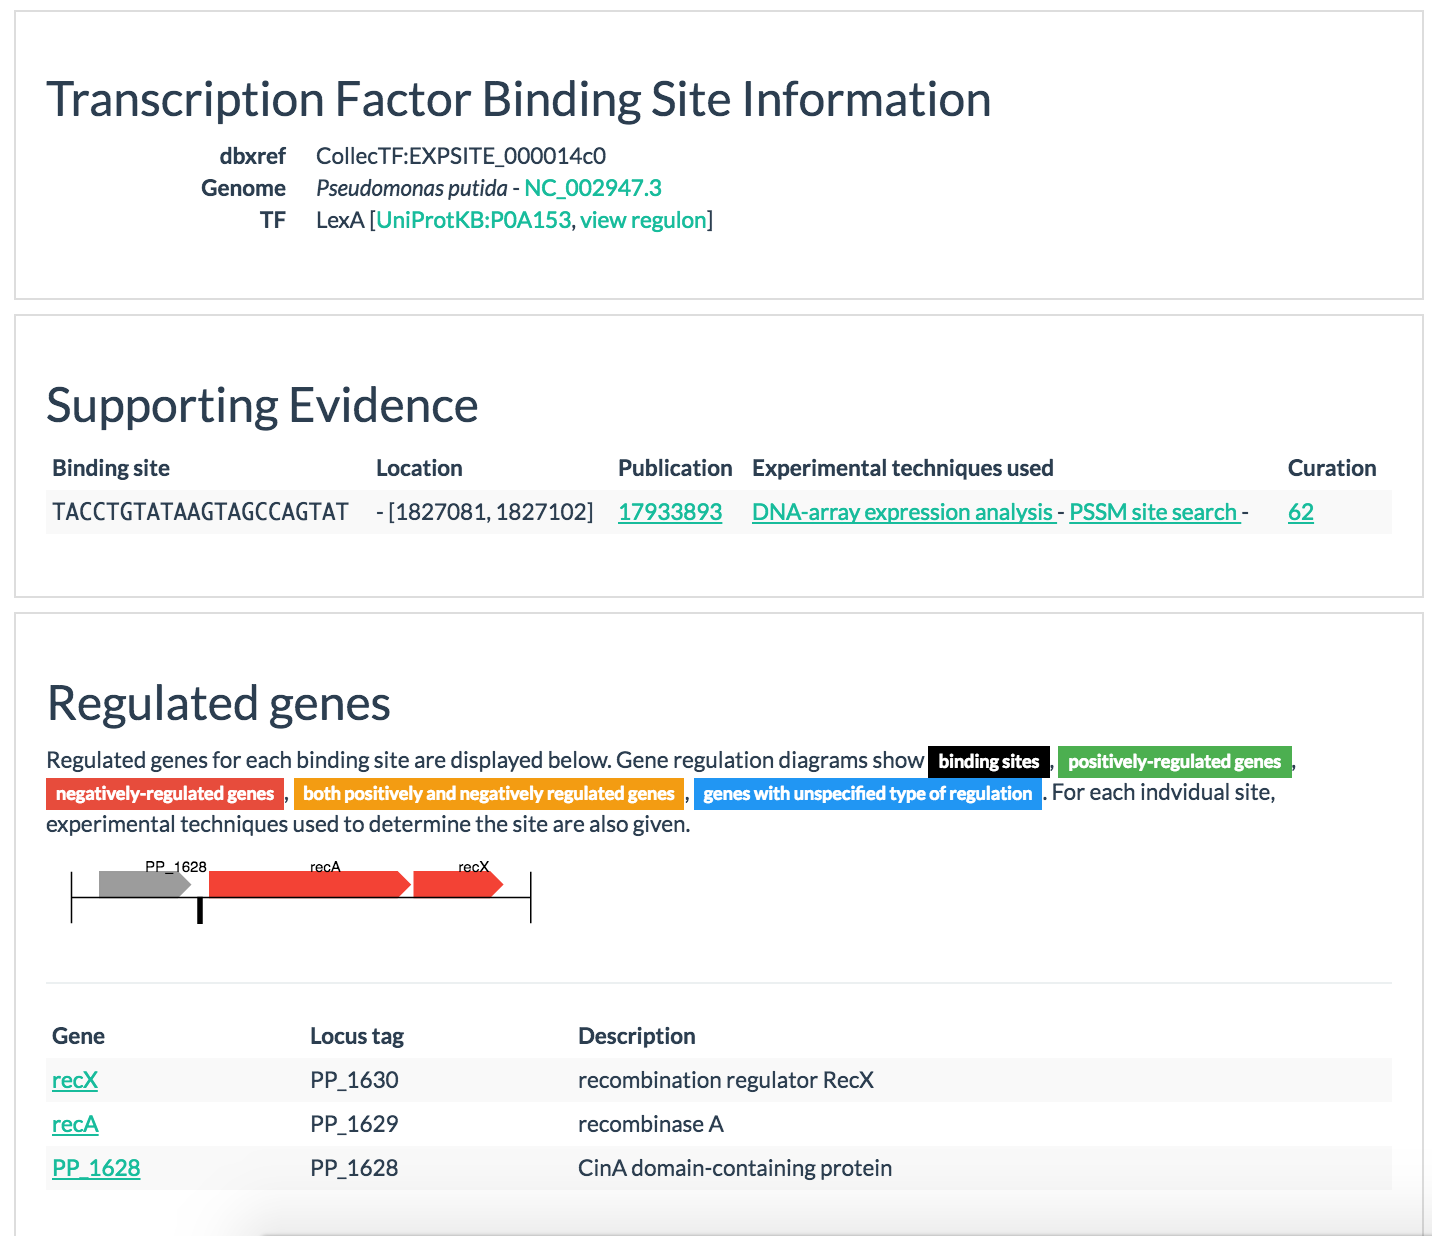
\includegraphics[width=\textwidth]{figures/chapter2/individual-site}
  \caption{Snapshot of the site report page for a \textit{Pseudomonas putida}
    LexA-binding site, illustrating the integration of supporting experimental
    evidence and including out-links to curations, publications, technique
    descriptions and NCBI Gene records. Like all other site report pages, this
    record is directly accessible through its \texttt{db\_xref} link at
    \url{http://collectf.org/EXPSITE_000014c0}.}
\label{fig:individual-site}
\end{figure}

\subsection{Motif comparison and genomic TF-binding site search}

A significant amount of work on transcriptional regulation mechanisms in
Bacteria focuses on the analysis of TF-binding motifs and their
evolution. CollecTF provides specialized tools to analyze TF-binding motifs in
different contexts. Pairs of TF-binding motifs, resulting from two independent
custom searches by the user, can be compared using a wide variety of methods,
such as an analysis of the pair-wise site Levenshtein distance within and
between motifs, the Kullback-Leibler divergence or the Pearson correlation
coefficient between motifs~\citep{vanet1999promoter, mahony2007stamp}. This
allows users to examine directly, for instance, the effects of different
criteria when requesting experimental support for TF-binding sites, or the
variability of TF-binding motifs across species and taxonomical groups
(Figure~\ref{fig:motif-comparison}). A canonical application of pre-fetched or
custom-generated collections of TF-binding sites is their use in TF-binding
site search and motif discovery algorithms. CollecTF provides a TF-binding
search service that allows users to search genome assemblies, as well as
integration with the MEME discovery suite as a reference database for
TF-binding site search and motif discovery~\citep{bailey2006meme}.

\begin{figure}
  \centering
  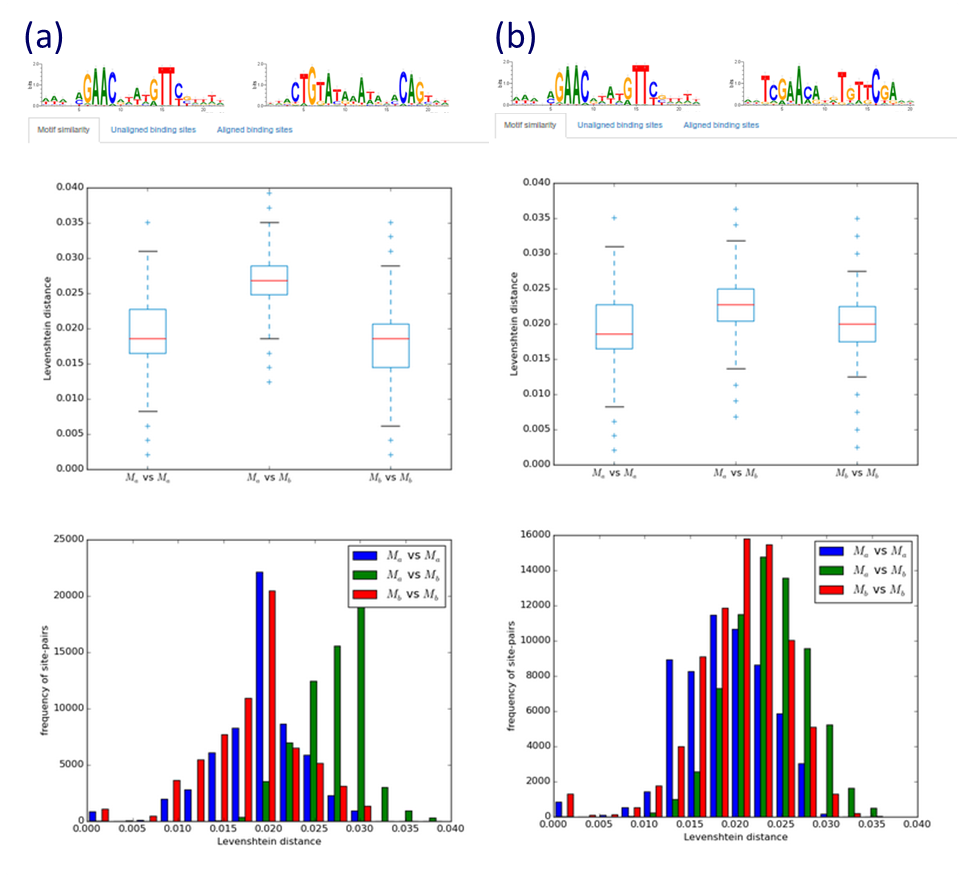
\includegraphics[width=\textwidth]{figures/chapter2/motif-comparison}
  \caption{Example of motif comparisons in CollecTF\@. Results of motif
    comparisons using the pair-wise site Levenshtein distance for: (a) the
    unrelated LexA-binding motifs of Firmicutes and Gammaproteobacteria and (b)
    the related LexA-binding motifs of Firmicutes and Actinobacteria. The
    analysis compares the pair-wise site Levenshtein distance between all site
    pairs within and between motifs and reports statistical differences among
    groups.}
\label{fig:motif-comparison}
\end{figure}

\section{Integration with major biological sequence resources}

Biological databases have rapidly become a cornerstone of modern biology,
centralizing access to knowledge and data to facilitate and often guide
experimental and computational research across all biological science
disciplines. Beyond major coordinated resources hosted by federal institutions,
such as the National Center for Biotechnological Information (NCBI) or the
European Bioinformatics Institute (EMBL-EBI), the biological database arena is
dominated by domain-specific databases~\citep{chen2007online,
  chandras2009models, bolser2012metabase, galperin20152015}. These databases
aggregate a community of researchers devoted to the highly-specific annotation
of a particular facet of biology (e.g.\ transcriptional regulation in Bacteria)
and have become an essential resource for biomedical research in many different
ways. Beyond compiling and making accessible highly-specific knowledge and data
to researchers in the field, these resources typically foster community
building and promote the development of standards, like controlled vocabularies
and ontologies~\citep{howe2008big, dunin2006modomics, schindelman2011worm,
  costa2013drosophila}. The wide variety and rapid proliferation of
domain-specific databases has generated a fragile ecosystem plagued by
diverging standards, short lifespans and lack of interoperability, making
information hard to access or gone when needed~\citep{wren2008databases}. Given
the time-intensive nature of the biocuration process, this “data tomb” effect
does not only have a direct repercussion on a database’s target domain, but
represents rather a net loss in public investment~\citep{merali2005databases,
  howe2008big, bastow2010sustainable}.

Proposed models for database financial sustainability are difficult to adopt
for databases addressing topics unattractive to private funders. They also tend
to restrict data sharing and limit community
participation~\citep{chandras2009models, bastow2010sustainable}. Hence, without
overt commitment by public agencies for long-term funding of domain-specific
databases, data and knowledge curated at great expense may face the risk of
becoming inaccessible due to proprietary restrictions or database demise. A
possible way out of such conundrum stems from the realization that the main
capital of domain-specific databases does not reside in the database and its
supporting infrastructure, but in the expertise and drive of a community of
researchers to annotate a particular facet of biology. Given this premise,
domain-specific databases can leverage the existence of central data
repositories to streamline their infrastructure, maximize the impact of
community expertise, focus their activity on meta-analysis and other
specialized services, and guarantee long-time accessibility to curated data.

Since its launch in 2013, CollecTF has been actively working to increase its
interoperability, visibility and long-term accessibility. In collaboration with
the NCBI RefSeq~\citep{pruitt2007ncbi}, CollecTF has streamlined the process for
direct annotation of RefSeq genome records. CollecTF has also established a
collaboration with the Evidence Ontology (ECO) to standardize its experimental
evidence terms and increase its
interoperability~\citep{chibucos2014standardized}, and set up collaborations
with the EMBL-EBI UniProt~\citep{uniprot2014uniprot} and Gene Ontology
Annotation (GOA) teams~\citep{ashburner2000gene} for the cross-referencing of
CollecTF records and the submission of Gene Ontology annotations. Hence,
CollecTF currently aims to contribute TF-binding site information not only in
the form of direct annotations on RefSeq genome records, but also as regulon
definitions for UniProt Knowledgebase (UniProtKB) protein records and
functional annotations of regulatory and binding mechanisms to the Gene
Ontology.


\subsection{Integration with NCBI RefSeq}

A significant fraction of database usage in biology involves access to large
derivative sequence repositories, such as the NCBI RefSeq and UniProt. Hence,
submission of domain-specific information to these resources does not only
guarantee long-term access to the data, but also maximizes its accessibility,
providing an incentive for direct author submissions. CollecTF compiles
information on experimentally-validated TF-binding sites. These are broadly
defined as segments of DNA that have been shown to be bound by a transcription
factor, and are typically involved in the regulatory function that the
transcription factor exerts on nearby genes. As such, TF-binding sites are
well-defined functional elements of the chromosome and hence amenable to
annotation on genome records. CollecTF annotates curated TF-binding site
information in complete RefSeq genome assemblies using the \verb|protein_bind|
feature identifier. The fields under this feature detail the location of the
TF-binding site, the protein accession for the transcription factor, the
experimental evidence for the annotation including PubMed identifiers for the
supporting publications and a \verb|db_xref| link to the original CollecTF
record (Figure~\ref{fig:dbxref}). The RefSeq submission process is now completely standardized
and has been upgraded to operate with the new non-redundant protein
sequences~\citep{o2015reference}. In agreement with the NCBI RefSeq, CollecTF
has focused initially on the targeted and exhaustive annotation of individual
genomes and, to date, it has populated 39 complete genomes with over 1,300
TF-binding site instances corresponding to more than 70 transcription factors,
providing for the first time comprehensive genome annotation of transcriptional
regulatory mechanisms for relevant bacterial clades, such as the
\textit{Vibrio} and \textit{Yersinia} genera and the Xanthomonadaceae and
Pseudomonadaceae families.

\begin{figure}
  \centering
  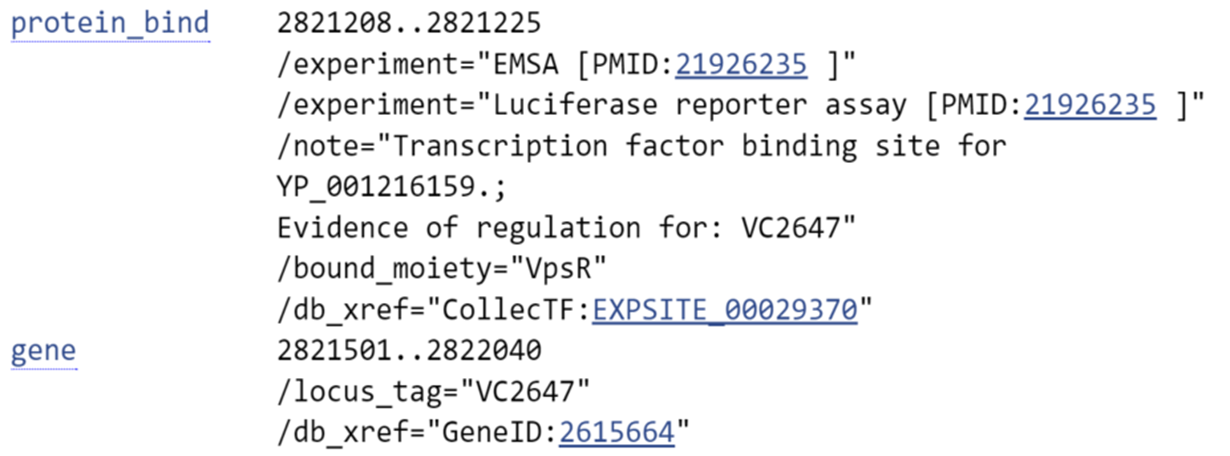
\includegraphics[width=0.8\textwidth]{figures/chapter2/dbxref}
  \caption{Excerpt from a RefSeq genome file (\texttt{NC\_002505.1},
    \textit{Vibrio cholerae} O1 biovar El Tor str. N16961 chromosome I)
    detailing the annotation of a binding site for the transcription factor
    VpsR. The annotation using the \texttt{protein\_bind} feature details the
    site location and the experimental techniques used to identify it, as well
    as direct links to the supporting literature. Genes regulated through
    TF-binding at the site, if known, are also reported, together with the
    binding protein using the \texttt{/bound\_moiety} field. The annotation
    also provides a \texttt{/db\_xref} outlink to CollecTF.}
  \label{fig:dbxref}
\end{figure}

\subsection{Integration with UniProt KnowledgeBase}

The sites bound by a transcription factor in a given genome constitute an
emerging property of the protein that can also be annotated in the protein
record. CollecTF generates specific records for all UniProtKB identifiers in
the database. These records encompass all available information on the binding
sites bound by the protein designated by the UniProtKB identifier and their
regulatory effects, and are cross-linked in the corresponding UniProtKB entry
through a \verb|db_xref| field. The CollecTF records for UniProtKB entries
contain detailed information on the sites bound by the TF, including their
genomic location, the experimental evidence and literature sources, the genes
regulated through the binding event and links to external databases providing
additional information on the binding mechanism (e.g.\ the Protein Data Bank),
the bound sites or their regulatory role (e.g. Gene Expression
Omnibus)~\citep{berman2000protein, barrett2005ncbi}
(Figure~\ref{fig:uniprot-integration}). The dual annotation of NCBI RefSeq
genome records and UniProtKB entries hence will provide a convenient way to
access the information available in CollecTF from the two constituting elements
of the TF-binding site interaction: the genome where the site is located and
the protein binding it. Furthermore, the integration of CollecTF with these
reference resources ensures its interoperability with other domain-specific
databases, maximizes the visibility of the data and its contributors, and
promotes long-term survival of the curated information.

\begin{figure}
  \centering
  \begin{subfigure}{0.7\textwidth}
    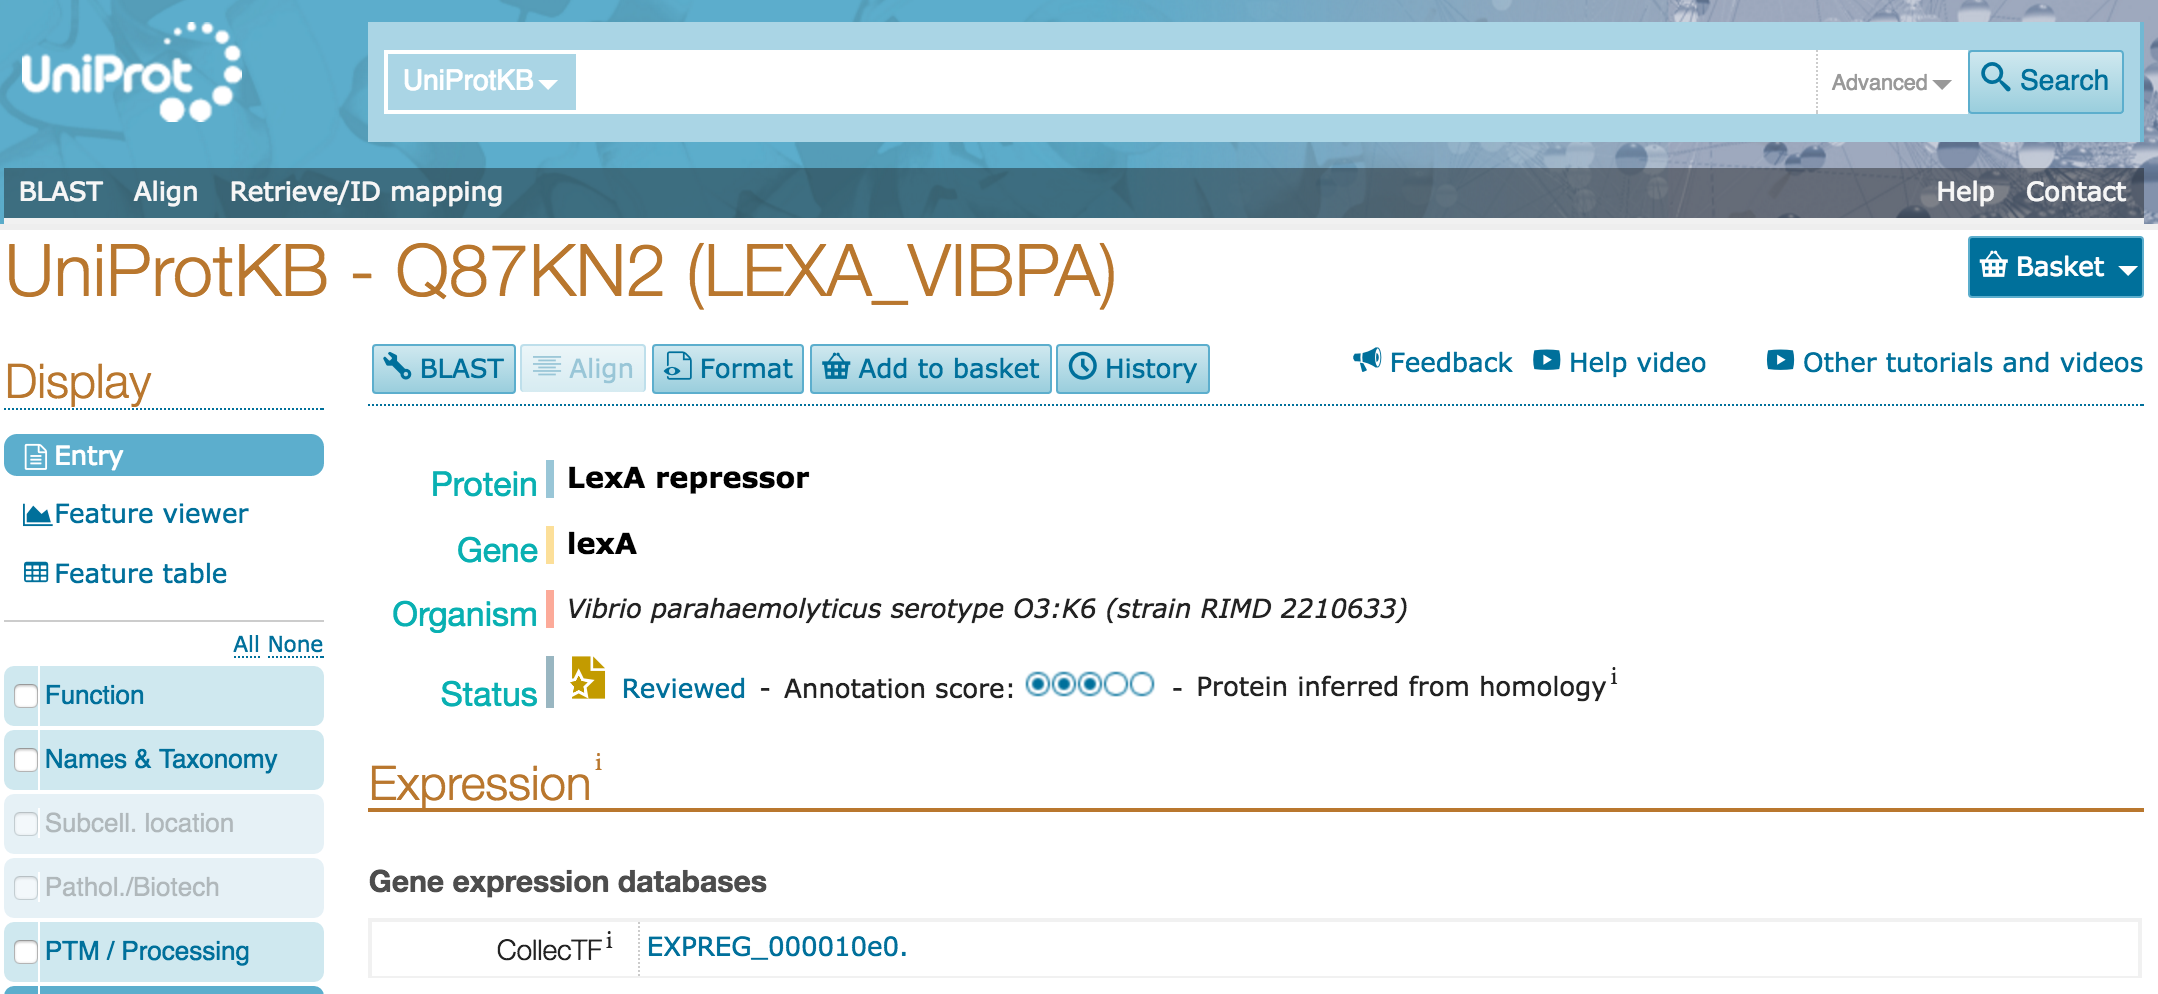
\includegraphics[width=1\textwidth]{figures/chapter2/uniprot}
    \subcaption{The Q87KN2 UniProtKB record, outlining the out-link to the
      CollecTF regulon record.}
  \end{subfigure}

  \begin{subfigure}{0.7\textwidth}
    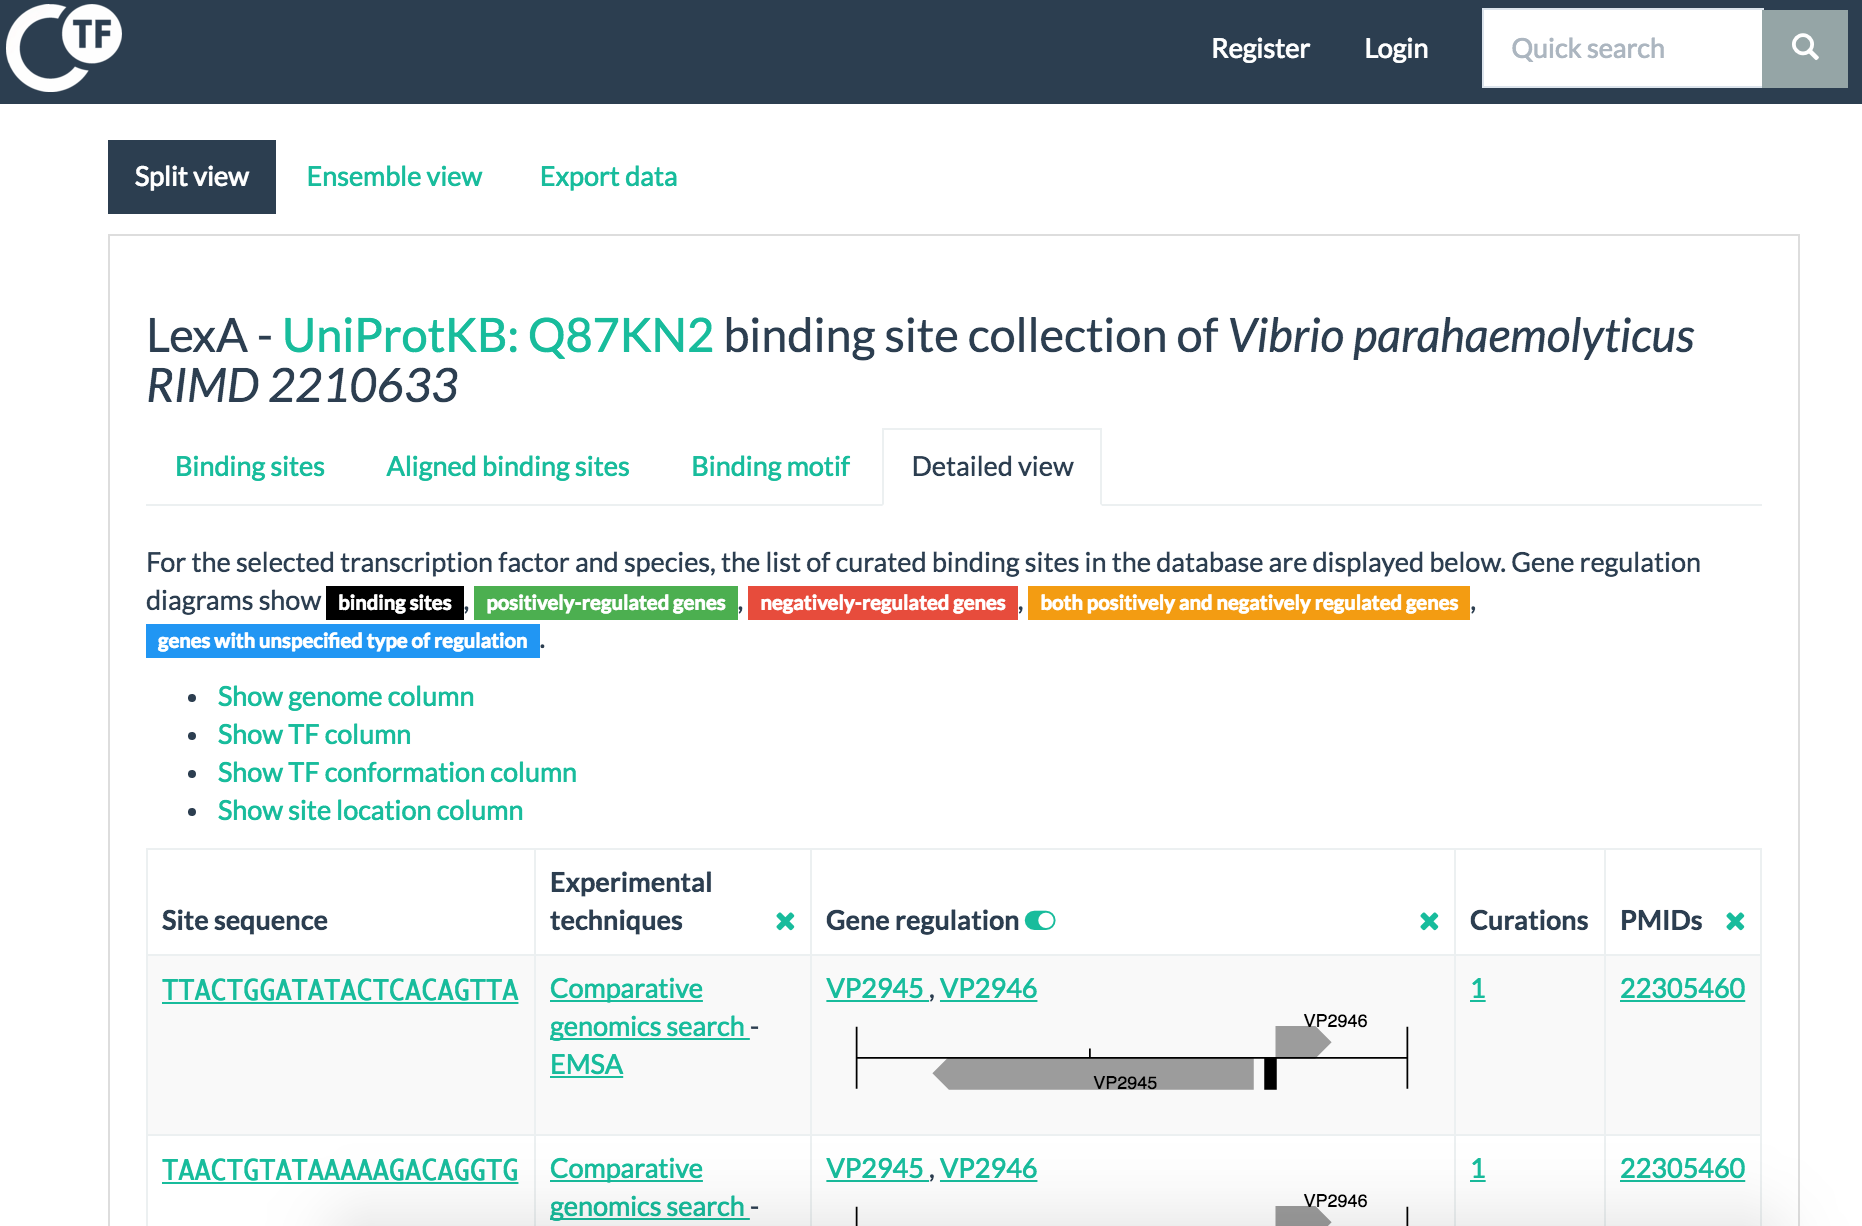
\includegraphics[width=1\textwidth]{figures/chapter2/protein-record}
    \subcaption{The CollecTF regulon record for Q87KN2}
  \end{subfigure}

  \caption{CollecTF record for UniProtKB entry Q9KU59.  UniProtKB report pages
    have multiple tabs, reporting binding sites before and after automatic
    alignment, a summary page containing the sequence logo generated from the
    multiple sequence alignment and motif statistics (motif structure,
    regulatory mode, TF conformation and site type), links to external
    databases and a detailed view. For each reported site, the detailed view
    provides the binding sequence, chromosome and protein accessions, the
    experimental evidence supporting its binding and regulatory effect, the
    reference literature sources, the genomic neighborhood highlighting (using
    a color code) regulated genes and a link to the curation record where users
    can find additional information on the experimental process.}
\label{fig:uniprot-integration}
\end{figure}

\subsection{Integration with Evidence Ontology}

By construction, the curation process in CollecTF defines relationships between
a gene product (the transcription factor), the genomic DNA it binds to and the
genes upon which such binding has a transcriptional regulatory effect. These
well-defined interactions can be captured by ontological statements using the
Gene Ontology (GO) formalism. A prerequisite for the generation of GO
annotations is the use of standardized terms for the experimental evidence
supporting them. To this end, CollecTF has worked in close collaboration with
the Evidence Ontology (ECO) team to map its controlled vocabulary of
experimental techniques to standardized ECO terms. This synergistic effort has
been extremely productive for both initiatives, increasing the interoperability
of CollecTF and leading to the creation and collaborative revision of new and
existing ECO terms.

\subsection{Submission of Gene Ontology annotations through GOA}
The CollecTF curation process implicitly yields two different types of
ontological statements. TF-centric statements capture the aspects of the
curation that establish different facets of the molecular function of the
transcription factor, such as its binding to DNA, with or without demonstrated
regulatory effect, or its regulation of transcriptional initiation for one or
more genes (Table~\ref{tab:go-terms}). TF-centric GO annotations are generated
automatically by the CollecTF curation pipeline, using the information provided
by the submitter during the curation process
(Figure~\ref{fig:gpad}). Gene-centric statements capture the involvement of
regulated genes in biological processes related to the transcription factor,
such as the response to DNA damage (GO:0006974) mediated in most bacterial
clades by the transcriptional repressor LexA~\citep{erill2007aeons}. Biological
processes related to a particular transcription factor are defined by curators
and assigned individually to regulated genes during the curation process. Upon
curation submission, this assignment is automatically encoded as a GO
annotation.


\begin{table}
\centering
\caption{Tabular schematic of the GO term identification guidelines for
  generation of TF-centric annotations in the CollecTF curation process. The
  guidelines define the GO terms to annotate given the experimental evidence
  reported in the curated literature.}
\label{tab:go-terms}
\renewcommand{\arraystretch}{1.4}
\begin{tabular}{l|l|C|C|C|C|C|C|C|C|}
  \cline{2-10}
  & \textbf{Annotation aspect} & \multicolumn{5}{l|}{Molecular function} & \multicolumn{3}{l|}{Biological process} \\
  \cline{2-10}
  & \textbf{GO term} & \rot{{GO:0043565}~} & \rot{GO:0001130} & \rot{GO:0001216} & \rot{GO:0001217} & \rot{GO:0000976} & \rot{GO:0006355} & \rot{GO:0045892} & \rot{GO:0045893} \\
  \cline{1-10}
  \multicolumn{1}{|l|}{\multirow{5}{*}{\textbf{\rot{\hspace{1em}Support for}}}} & DNA sequence binding activity & \x & \x & \x & \x & \x & \x & \x & \x \\
  \cline{2-10}
  \multicolumn{1}{|l|}{} & Regulation of expression (generic) &  & \x &  &  & \x & \x &  & \\
  \cline{2-10}
  \multicolumn{1}{|l|}{} & Regulation of expression (activation) &  &  & \x &  & \x & &  & \x\\
  \cline{2-10}
  \multicolumn{1}{|l|}{} & Regulation of expression (repression) &  &  &  & \x & \x &  & \x & \\
  \cline{1-10}
\end{tabular}

\bigskip

\begin{tabular}{|l |p{13cm}|}
\hline
GO term & Definition\\
\hline
\hline
GO:0043565 & sequence-specific DNA binding\\
\hline
GO:0001130 & bacterial-type RNA polymerase transcription factor activity, sequence-specific DNA binding\\
\hline
GO:0001216 & bacterial-type RNA polymerase transcriptional activator activity, sequence-specific DNA binding\\
\hline
GO:0001217 & bacterial-type RNA polymerase transcriptional repressor activity, sequence-specific DNA binding\\
\hline
GO:0000976 & transcription regulatory region sequence-specific DNA binding\\
\hline
GO:0006355 & regulation of transcription, DNA-templated\\
\hline
GO:0045892 & negative regulation of transcription, DNA-templated\\
\hline
GO:0045893 & positive regulation of transcription, DNA-templated\\
\hline
\end{tabular}

\renewcommand{\arraystretch}{1}

\end{table}

TF- and gene-centric GO annotations stemming from validated curations are
automatically appended to the CollecTF GPAD file~\citep{gene2013gene},
accessible through a static CollecTF
URL\footnote{\url{http://collectf.org/static/collectf.gpad}}. GO annotations
generated by CollecTF will be periodically collected by the EMBL-EBI Gene
Ontology Annotation (GOA) team from this static URL and reviewed before
submission to the Gene Ontology Consortium.


\begin{figure}
  \centering
  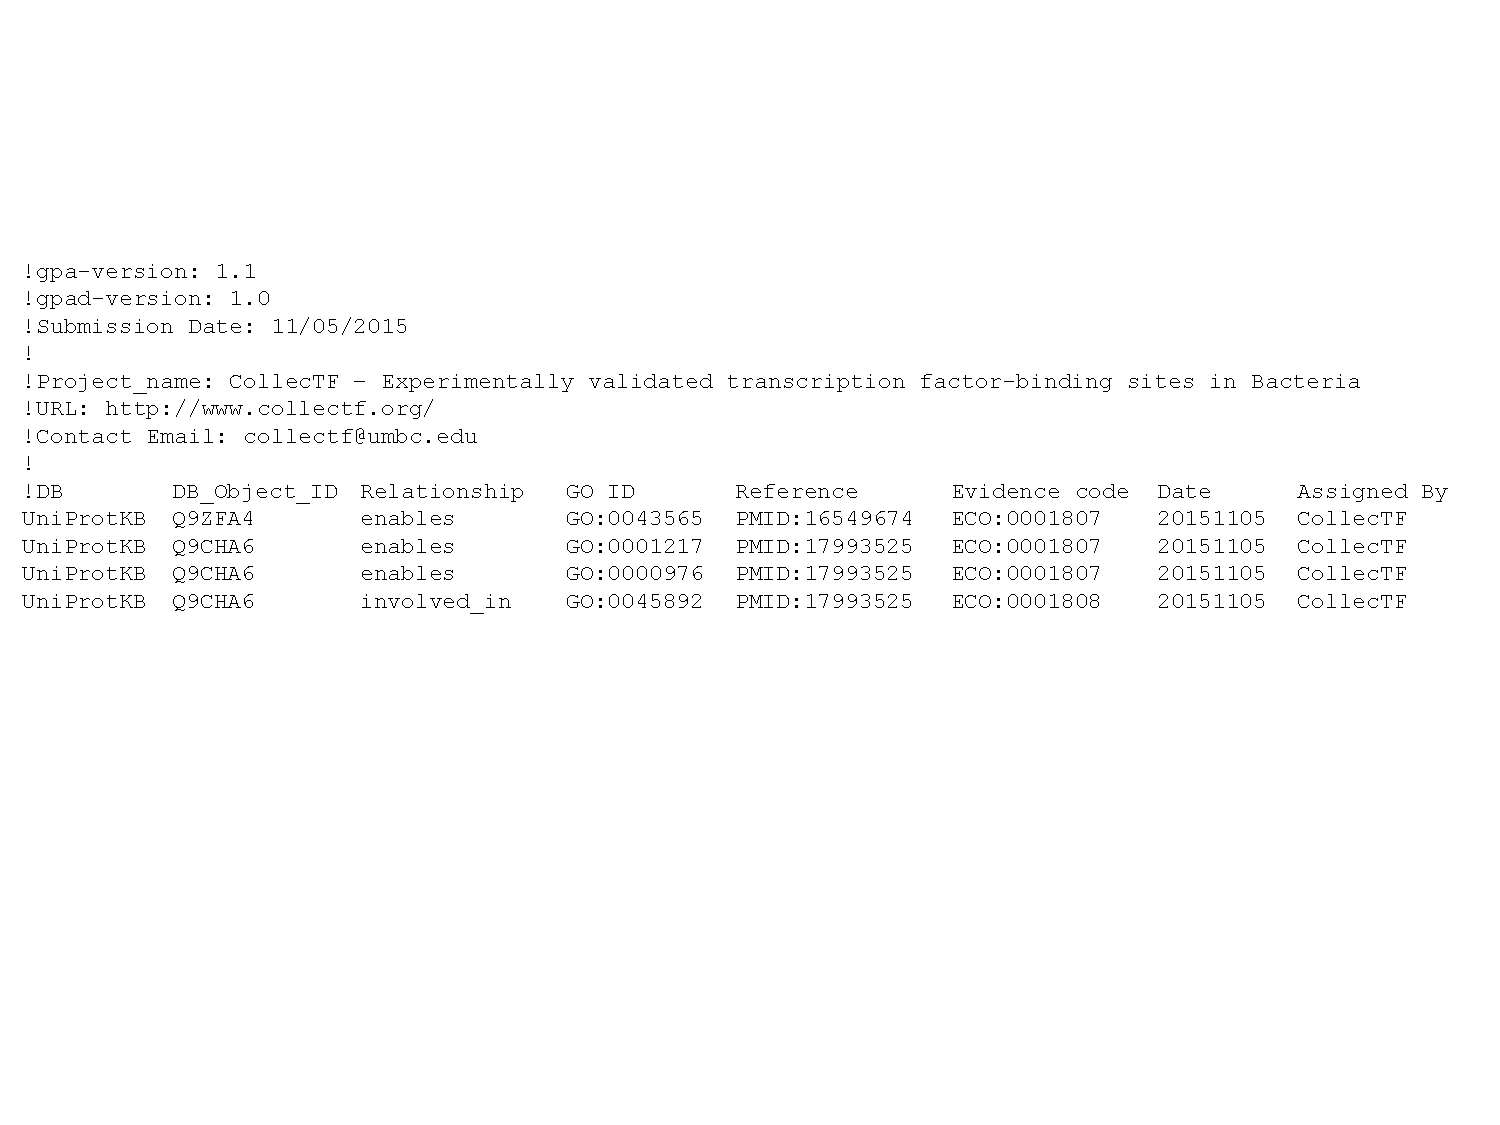
\includegraphics[width=\textwidth]{figures/chapter2/gpad}
  \caption{Excerpt from the GPAD-formatted file generated by CollecTF, showing
    TF-centric annotations corresponding to two curations. Each individual line
    represents an annotation, with the relationship field denoting whether the
    gene product specified by the UniProtKB identifier enables a molecular
    function or is involved in a biological process. The specific function
    supported by the evidence is defined by a GO ID, such as GO:0001217
    (bacterial-type RNA polymerase transcriptional repressor activity,
    sequence-specific DNA binding). The literature reference is indicated by
    means of a PubMed ID, and the evidence supporting the annotation is
    specified by an Evidence Ontology term, such as ECO:0001807
    (electrophoretic mobility shift assay evidence used in manual assertion).}
\label{fig:gpad}
\end{figure}